\documentclass{article}

\usepackage{CJKutf8}

\usepackage{listings}
\usepackage{xcolor}
\lstset { %
	language=C++,
	backgroundcolor=\color{black!5}, % set backgroundcolor
	basicstyle=\footnotesize,% basic font setting
}

\usepackage{graphicx} %package to manage images
\graphicspath{ {images/} }

\title{SLAM Theory and Practice: Home Work 1}
\author{Liang Xu \\ liangxucs@gatech.edu}
\date{February 2018}

\begin{document}
\begin{CJK*}{UTF8}{gbsn}
\maketitle

\section{熟悉 Linux}
\subsection{如何在 Ubuntu 中安装软件(命令行界面)?它们通常被安装在什么地方?}
	apt-get install {package name}\\
	Most of the user program saved in /usr/bin ----> binary file\\
	Sometime saved in /opt if the bin too big
\subsection{linux 的环境变量是什么?我如何定义新的环境变量?}
Linux 环境变量是指, Linux 运行环境的一些参数,比如说,临时文件的位置,bin file 的路径 等。\\
Add the new environment variable to /etc/profile for all user\\
Add to /.bashrc for current user.

\subsection{linux 根目录下面的目录结构是什么样的?至少说出 3 个目录的用途}
/bin :contains executable programs which are needed in single user mode\\
/etc :Contains configuration files which are local to the machine.\\
/home: home directories for users. \\
/lib: shared libraries\\
/mnt : mount point \\
/root:home for root user.\\ 
/usr: hold sharable, read only data. 

\subsection{假设我要给 a.sh 加上可执行权限,该输入什么命令?}
sudo chomd +x a.sh

\subsection{假设我要将 a.sh 文件的所有者改成 xiang:xiang,该输入什么命令?}
sudo chown xiang:xiang a.sh

\section{SLAM Literature Survey}
\subsection{SLAM 会在哪些场合中用到?至少列举三个方向。}
1. Can be used in the robotic vehicle to locate the current position and map the current map.\\
2. Use the Augmented Reality(AR) to merge the virtual and real environment. \\
3. 3D scene reconstruction by multiply image. 

\subsection{SLAM 中定位与建图是什么关系?为什么在定位的同时需要建图?}
Because the sensor data always have noise part. So, no matter how accuracy the sensor is, the accumulated error will come up. SLAM solves this problem by correcting the current location and remapping the environment. The current mapping gives the prior information for the next measurement step for batter position estimation. Current measurement and location can help to rebuild more accuracy map. \\
The map often required for other task, for example, path planning. The map also can limit the error to estimate the current sensor position. 

\subsection{SLAM 发展历史如何?我们可以将它划分成哪几个阶段?}
SLAM has been widely used in the robotic field in the past several decade. And the history can be dividend by 2 phases: 
classical age(1986-2004), the classical age mainly cover the probabilistic formulations. 
algorithm-analysis age(2004-2005), the study of fundamental properties of SLAM. 

\subsection{列举三篇在 SLAM 领域的经典文献}
1. Simultaneous Localization and Mapping: Part I , Part II \\
2. MonoSLAM: Real-Time Single Camera SLAM \\
3. FastSLAM: A factored solution to the simultaneous localization and mapping problem

\section{CMake Practice}
\begin{lstlisting}
cmake_minimum_required( VERSION 2.8 )

project( HelloSLAM )
set( CMAKE_BUILD_TYPE "Release" )

include_directories("include")
add_library(hello SHARED src/hello.cpp)

add_executable(useHello useHello.cpp)
target_link_libraries(useHello hello)

install(TARGETS hello DESTINATION "/usr/local/lib/")
install(FILES include/hello.h DESTINATION "/usr/local/include/")
\end{lstlisting}


\section{理解 ORB-SLAM2 框架}
\subsection{Download}

\begin{figure}[h]
	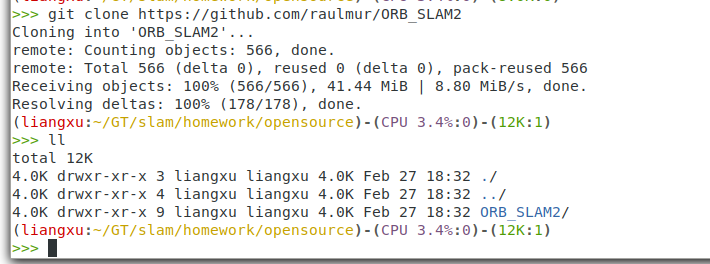
\includegraphics[width=8cm]{download_verf.png}
	\centering
\end{figure}

\subsection{Answer Questions}
\subsubsection{ORB-SLAM2 将编译出什么结果?有几个库文件和可执行文件?}
compile 19 library files in src/ and link those library with opencv, eigen3, pangolin,DBoW2 and g2o. Complication will generate six executable files and saved in the /Example/** folder. 

\subsubsection{ORB-SLAM2 中的 include, src, Examples 三个文件夹中都含有什么内容?}
include have all the header file, and src have all the source code. Example folder contains different examples for using this research project. 

\subsubsection{ORB-SLAM2 中的可执行文件链接到了哪些库?它们的名字是什么?}
OpenCV, computer vision\\
eige3, for matrix computation\\
Pangolin, for display\\

\section{使用摄像头或视频运行 ORB-SLAM2}
\subsection{compilation finish}
\begin{figure}[h]
	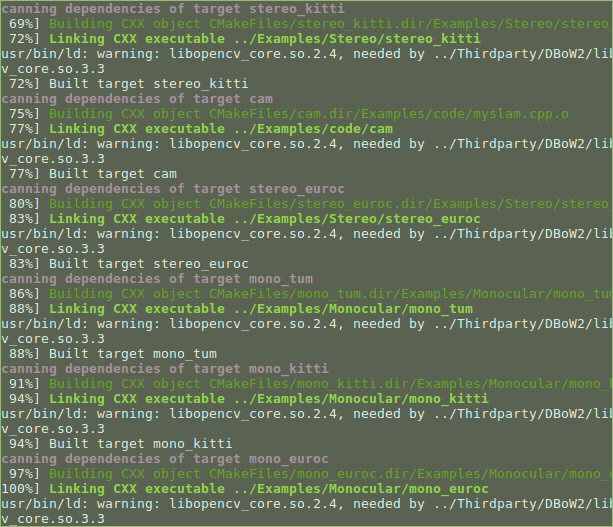
\includegraphics[width=6cm]{compile.png}
	\centering
\end{figure}

\subsection{CMakeLists.txt 修改方案}
move the code\ folder under Example\ Then add the following code to CmakeList.txt. Two executable files will be created, one is for recorded video called video, another is for the video camera, called cam. 

\begin{lstlisting}

set(CMAKE_RUNTIME_OUTPUT_DIRECTORY ${PROJECT_SOURCE_DIR}/Examples/code)
add_executable(video
Examples/code/myvideo.cpp)
target_link_libraries(video ${PROJECT_NAME})

add_executable(cam
Examples/code/myslam.cpp)
target_link_libraries(cam ${PROJECT_NAME})

\end{lstlisting}

\subsection{Result}
CMake give us a very robust compilation environment setup. 
\begin{figure}[h]
	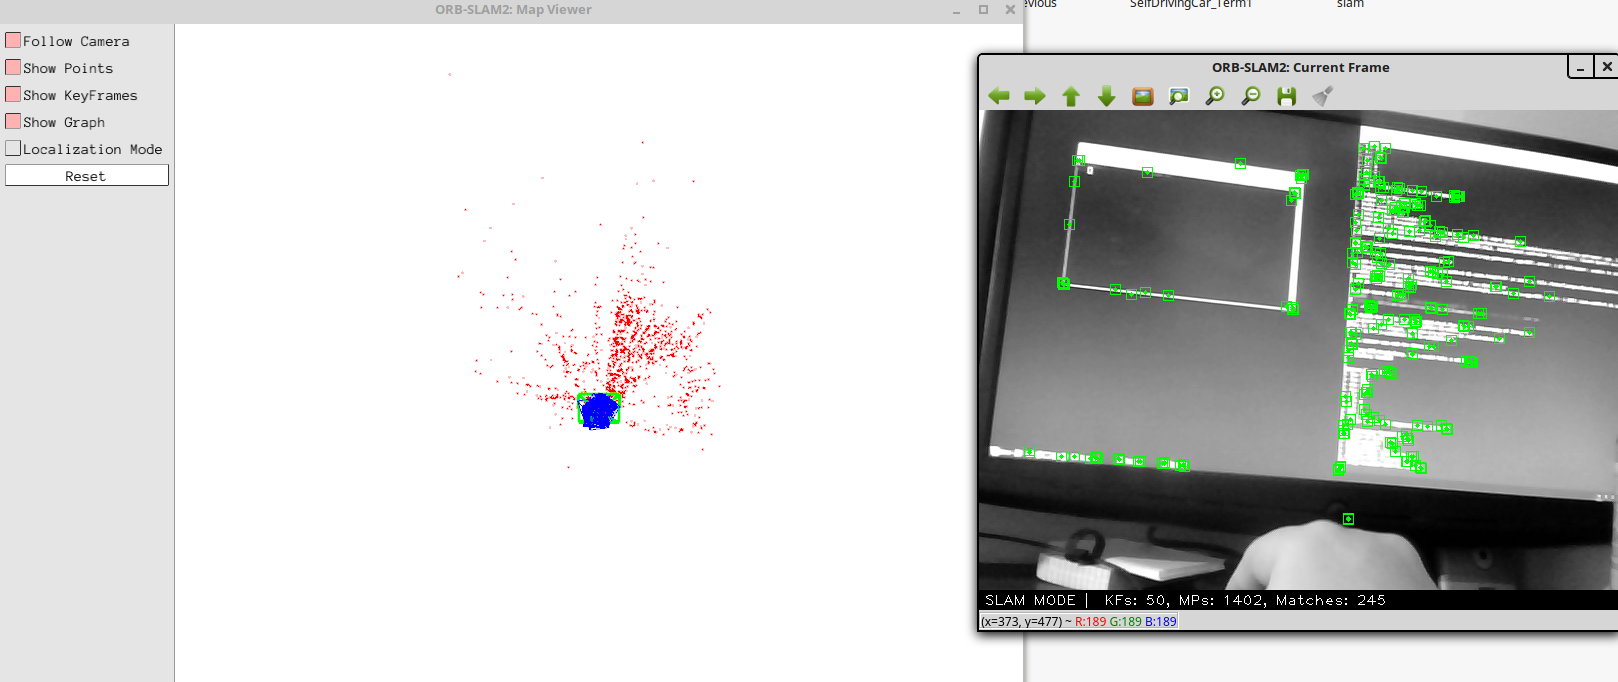
\includegraphics[width=8cm]{camerara.png}
	\centering
\end{figure}

\clearpage\end{CJK*}
\end{document}
